\documentclass[
	%a4paper, % Use A4 paper size
	letterpaper, % Use US letter paper size
]{jdf}

\addbibresource{references.bib}

\author{Nan Xiao}
\email{nanx@gatech.edu}
\title{CS6750 HCI Summer 2021:\\Assignment M5}

\begin{document}
%\lsstyle

\maketitle

\begin{abstract}
	LinkedIn is one of the most popular social networks for professionals. Many of us rely on LinkedIn to expand connections and find new opportunities after graduation. In this project, we are going to study one task of LinkedIn - the searching function. The objective is to make a better interface design that the users can have a more relevant result on the LinkedIn search result page and accomplish the task.
\end{abstract}

\section{Qualitative Evaluation}
\subsection{Evaluation report}
As planned in M4, we are using interviews to evaluate the Wizard of Oz prototype - using the voice signature to identify who you are talking with. Here is a quick recap of what the prototype looks like. As shown in Figure 1, when a user is talking to another person, the interface should be able to use the voice signature to identify the person's LinkedIn profile and make the suggestion to the user.
\begin{figure}[h]
	\centering
	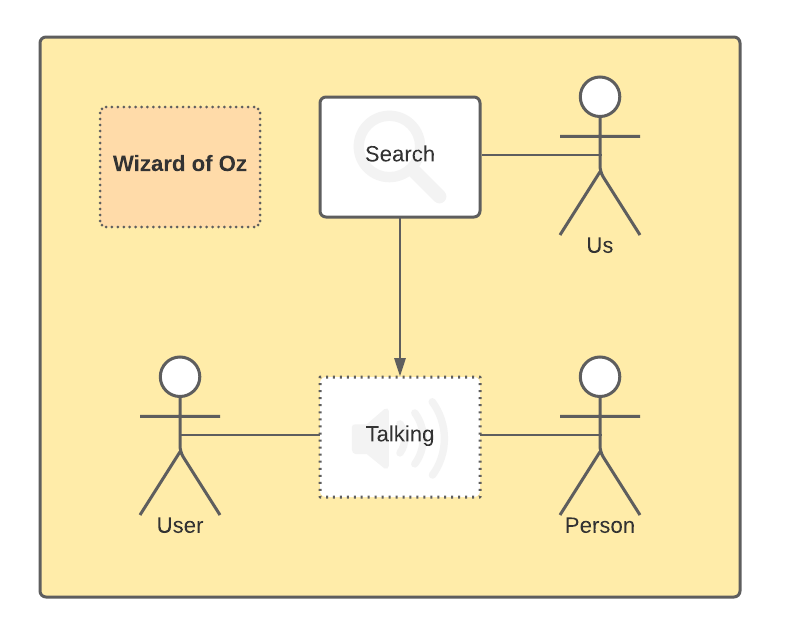
\includegraphics[height=5cm]{jdf-latex/Figures/Wizard of Oz.png}
	\caption{Wizard of Oz prototype for identify who you are talking to}
	\label{fig:wizard}
\end{figure}

\subsection{Raw Results}
15 people are interviewed during this evaluation. The interview questions are in the appendices. Below are the raw results from the interviews.
\begin{enumerate}
    \item \textbf{8 of 15} people would like to know the LinkedIn profile of the person they are talking with. Feedback is that most of the time it happens on professional occasions.
    \item \textbf{10 of 15} people find themselves spend much time searching people using different combinations of names and filters.
    \item \textbf{14 of 15} people find it helpful to search for someone without even knowing the name.
    \item \textbf{9 of 15} people will search LinkedIn while \textbf{6 of 15} will ask directly when people want to know where their new colleague worked before?
    \item \textbf{13 of 15} people think it is very helpful if instead of you initiate the searching, the LinkedIn app can suggest the profile of the person you are talking with.
    \item \textbf{11 of 15} people think the main concern is privacy, they do not want to be searched by a stranger.
    \item (If yes for the above question), \textbf{9 of 11} people think turning off searchability will solve this issue.
    \item \textbf{15 of 15} people think this interface should be on the mobile device.
\end{enumerate}

\subsection{Feedback Analysis}
From the above result, we can see that, there is a strong need for people to search for people they do not know names on professional occasions. It is like a more convenient way of exchanging name cards in the old days. Also, recommend users based on the sound bridge the gulf of executions as well, the user is essentially evaluating the result straightaway. The biggest concern is still privacy, no one would like to be searched for working information by strangers. But with appropriate security features in place, the users are OK with the new interface. The interface is particularly helpful in certain scenarios like meeting with new colleagues or attending professional conferences. There can be features to allow the interface to be turned on in certain locations.

\subsection{Potential Changes Feedback}
Based on the strong signal from the interviews, the interface should be focused on delivering the best mobile experience. To mitigate the privacy concerns, security features like allowing users to turn off searchability need to be added to the interface.

\section{Predictive Evaluation}
\subsection{Recap of the prototype}
As planned in M4, we are using the cognitive walkthrough to evaluate the wireframe prototype - using a photo to do facial recognition and match the LinkedIn profile. Here is a quick recap of what the prototype looks like. As shown in Figure 2, a user can upload a photo instead of searching for a name. The interface then should be able to use the facial recognition model to identify the most relevant LinkedIn profiles.

\begin{figure}[h]
	\centering
	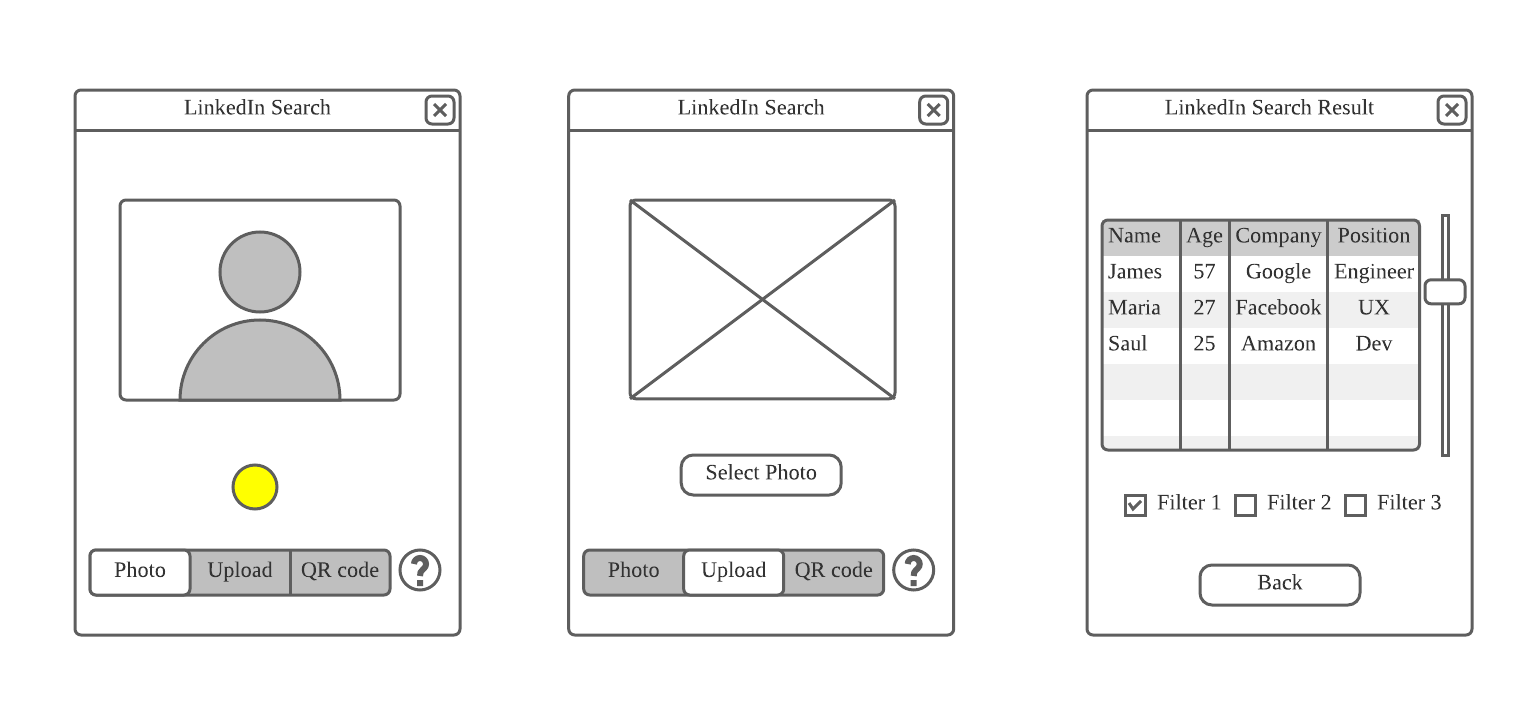
\includegraphics[height=5cm]{jdf-latex/Figures/LinkedIn Search Prototype.png}
	\caption{Wireframe of facial recognition in LinkedIn search function}
	\label{fig:wireframe}
\end{figure}

The \textbf{goal} of the user is to find the correct LinkedIn profile of the photo uploaded. It can be a single photo, a group of photos, or taking a real-time photo. The interface will be able to match that photo to the database and find the corresponding LinkedIn profiles of people in the photo.
\subsection{Cognitive Walkthrough}
Cognitive task analysis adopts the predictor view of a human's role in the system. It generally follows below common sequence: (\cite{joyner2016})

\begin{enumerate}
	\item Collecting preliminary knowledge
	\item Identify knowledge representations
	\item Apply focused knowledge elicitation methods
	\item Analyze and verify data acquired
	\item Format results for the intended application
\end{enumerate}

\textbf{Top level task} - Find someone's LinkedIn profile using its photo
\begin{itemize}
    \item \textbf{Sub-task} - Uploading the photo for searching the LinkedIn profile
        \begin{itemize}
            \item Operator - Clicking the LinkedIn search box
            \item Operator - Clicking Upload tab
            \item Operator - Clicking Select Photo
            \item Operator - Uploading the photo
        \end{itemize}
    \item \textbf{Sub-task} - Taking a real-time photo for searching the LinkedIn profile
        \begin{itemize}
            \item Operator - Clicking the LinkedIn search box
            \item Operator - Clicking Photo tab
            \item Operator - Clicking the yellow button to take a photo 
        \end{itemize}
    \item \textbf{Sub-task} - Find the correct profile in the search result page
        \begin{itemize}
            \item Operator - Scroll the page to find the result
            \item Operator - Use filters to find the result
            \item Operator - Go back to last page
        \end{itemize}
    \item \textbf{Design principle - consistency}
        \begin{itemize}
            \item Using the similar interface as photo app for user to upload photos
            \item Using the similar interface as photo app for user to take photos
            \item Operator - Go back to last page
        \end{itemize}
    \item \textbf{Design principle - simplicity}
        \begin{itemize}
            \item User can only take photos or upload photos to search, the interface is minimized to focus on these 2 tasks.
            \item Results page contains only necessary information, only name, age, company and position are shown.
        \end{itemize}
    \item \textbf{Design principle - tolerance}
        \begin{itemize}
            \item Photos from most angles are acceptable, 90 degree front photo is not required.
            \item Even with low light condition, the app can still recognize the photo.
            \item Hair style or outfits will not affect the accuracy.
        \end{itemize}
    \item \textbf{Design principle - affordance}
        \begin{itemize}
            \item User will understand the interface is mean to take a photo
            \item The checkbox design and scroll bar design will let user understand how to navigate in the result interface
            \item The question mark design will let user understand this is the button to look for help
        \end{itemize}
    \item \textbf{Design principle - mapping}
        \begin{itemize}
            \item The interface maps the experience that you recognize a person through the appearance
        \end{itemize}
    \item \textbf{Design principle - perceptbility}
        \begin{itemize}
            \item The user can see the photo immediately after uploading or taking.
            \item The user can get immediate response about the relationship between the photo provided and results. Better photo will give a more accurate result.
        \end{itemize}
\end{itemize}

\section{Evaluation Summary}
\subsection{Information to understand about the user more fully}
Additional needfinding exercises need to be conducted to collect scenarios that users are using the LinkedIn searching box. We may need to combine all the prototypes and use different interfaces according to the user scenarios. For example, when users are talking to other professionals in the conference, the interface based on sound signature is used. And when the user is searching for a schoolmate based on the Instagram photo, the photo searching interface is used. We need to collect more user journeys to understand how to design better interfaces according to those scenarios.

Questions arose based on the evaluation that needs further investigation separate from the prototypes themselves:
\begin{enumerate}
    \item What are the most common scenarios that you need to use the LinkedIn search box on mobile?
    \item What are the most common scenarios that you need to use the LinkedIn search box on a laptop or desktop?
    \item What are the different privacy concerns when you are using the LinkedIn search box in different scenarios?
\end{enumerate}

\subsection{Additional Design Alternatives}
Through the feedback, we can understand that for the same task, same user, but different context, people may need a different interface or the interface should consider the context. So participant view of the user is more applicable in our case. Especially for privacy concerns, people are OK with the new interface in the familiar context like workplace or friend's home. But they do not want to be searched on LinkedIn on public transport or libraries. We will add additional context-based security features in the next iteration of the design life cycle.

\subsection{Revisions to the prototypes to make}
First, we will bend the different prototypes into one interface, with additional security designs. This will address most of the concerns from the feedback. Second, the prototype will be moved to the next level of fidelity, thus we can have more accurate feedback about the user experience. Using wireframes, users are more focused on the functionality. But with a higher fidelity prototype, we can collect feedback on the user interface as well.

\begin{table}[h] % [h] forces the table to be output where it is defined in the code (it suppresses floating)
	\caption{Design Alternatives and Revisions}
	\small % Reduce font size
	\centering % Centre the table
	\begin{tabular}{L{0.3\linewidth} L{0.3\linewidth} L{0.3\linewidth}}
		\textbf{Feedback} & \textbf{Design Alternatives} & \textbf{Revisions} \\
		\toprule[0.5pt]
		Different scenarios may need different interfaces & Bend the different interface into one and choose based on context & - \\
		\midrule
		Security concern, the user do not want always be searchable & Introduce the feature to turn off the profile & Higher fidelity to collect user feedback of security feature \\
	\end{tabular}
\end{table}

\subsection{Plan of evaluation to employing next}
In the next iteration of the design life cycle, we will conduct another round of needfinding exercises to get more context when users are using the LinkedIn search function. Also, we will combine the existing prototypes and introduce new security features. Thus qualitative evaluation is still important because we will be changing the app in many domains. With a high fidelity interface that allows users to interact, we may consider introducing quantitative evaluation as well to compare which kind of security feature design is more acceptable to the users.


\section{References}
\printbibliography[heading=none]

\section{Appendices}
\textbf{Interview Questions:}
\begin{enumerate}
    \item How often would you like to know the LinkedIn profile of the person you are talking with?
    \item How often do you forget your connections and spend much time searching people using different combinations of names and filters?
    \item How helpful would it be if you can search for someone without even knowing the name?
    \item What would you do if you want to know where your new colleague worked before?
    \item Would it be helpful if instead of you initiate the searching, the LinkedIn app can suggest the profile of the person you are talking with?
    \item What could be your concern if the LinkedIn search function can help you to identify who you are talking with?
    \item (If yes for the above question), do you think if you are allowed to turn off searchability of your profile can help to mitigate the privacy concern?
    \item On which device would you prefer to see this function?
\end{enumerate}

\end{document}